\chapter{Analysis and Design}
In this chapter, we will describe and justify the design of our
library and the thoughts and considerations that went into producing
the final design and ideas that was discarded along the way. We will
primarily focus on how the SME model can be parallelized.

%\section{Overall goal and success parameters}

% \section{Programming}
% Even though the eventual goal of the SME-library is to enable
% generated networks to execute
% The API exposed to the user of the SME library should be designed with
% a focus on balancing expressiveness and ability to be easily
% understandable....

% The API implemented by \cite{vinter2014synchronous} is heavily
% dependent of the highly dynamic nature of the Python programming
% language used to implement their prototype. Since our implementation
% is written in C++ we cannot directly mimic the python API in our
% implementation. Given the similarities between SME and CSP it seems
% obvious to let us inspire by

\section{Paralellization model}
A common way of parallelizing CSP-like networks is to use user-level
threads to represent a process. In comparison with OS-level threads,
user-level threads has a significantly lower overhead both with
regards to context switching penalty \cite{sung2002comparative} and
memory cost. Furthermore, a  much higher number of user-level threads can
coexist on a system. Due to these limitations, implementing these kind of
message passing systems using only OS-level threads are generally not
feasible. Therefore, user-level threads are used by other message
passing systems such as the C++CSP library\cite{brown2003introduction}
and the goroutines in the Go
language\cite{deshpandeanalysis}. However, implementing a user-level
threading library would add complexity to our program since we would
need to implement a scheduler, for scheduling processes on top of
OS-level threads.

Comparing, once again, to CSP, the concurrency in CSP is inherently
asynchronous while SME is entirely synchronous in nature. This means
that a CSP library needs to implement a scheduler which decides when
to give control to a process based on certain events, e.g. a process
wishing to communicate or a process receiving a message from another
process.

We initially considered a similar design for C++SME, however, due to
the enforced synchrony of SME we don't have the same need to schedule
processes ``intelligently'' since we know that, during a cycle, all
processes needs to run and all busses have to propagate their
values. This, in addition to the shared nothing property of SME, allows
us to specify a much simpler parallelization model for SME compared to
the techniques used by the aforementioned message passing network
implementations.

The basic idea that we base our design on is conceptually similar to a
classic producer-consumer setup. In our case, the work ``produced''
are pointers to the processes in the network, and the consumers are the threads
executing the processes. In this setup, a process is executed by a
simple function call. Once again, this simplifies our implementation
compared to an equivalent implementation using user-level threads.

%This, once again, simplifies  our
%implementation compared to using whereas user-level threads are usually implemented
%using the \texttt{setcontext} and \texttt{getcontext} library
%functions, which, while extremely fast, still causes a slightly larger
%overhead compared to a simple function call.

%\fxnote{Switching between
%  OS-level processes is actually really fast, since context-switching
%  from one process to another usually only involves moving CPU
%  registers, i.e. the stack pointer, to an appropriate location, TODO
%  write something like that}

%by simply letting a number of OS-threads run SME processes in a
%worker-consumer like manner. This approach also make it simple enforce
%the synchrony property of SME, since

In this project, we have explored two different variations of this
basic idea. Both models are based on the idea described in the
previous paragraph. Our overall goal in parallelizing execution of
SME-networks is to minimize the amount of core idle time. We expect
the hereafter presented models to achieve this goal under different
circumstances.



%\subsection{Pros and cons}
%Pros: Shared nothing,forced synchrony 

%Cons: Forced syncrhony 

%\subsection{``Worker queue'' model}
\subsection{Work list model}
This approach most closely matches the aforementioned producer-consumer model where we
have a number of workers which takes tasks off a circular queue and
executes them. This model executes processes in a
"round-robin"-like manner allowing it to "interlace" processes
with different computational loads. Thus, we expect that this model to
produce lower overall execution times for networks with uneven
workloads (\cref{fig:worklist}). The primary problem of this model is
that we need to make the queue thread-safe. The locking mechanism
needed to do this isn't free and could therefore become a dominant
factor in the execution speed of networks consisting of many (small)
processes.

When shortness is needed, we will refer to this model as Model 1 or
M1.

\begin{figure}
\centering
\includegraphics{figures/roundrobin}
\caption[Work list model]{Illustration of the work list model. The
  order of which processes are executed is shown as dashed arrows of
  increasing density}
\label{fig:worklist}
\end{figure}


%Processes will be executed on the first available core as seen in
%\cref{fig:worklist}

\subsection{Static orchestration model}
In this model, we assign separate queues to each thread of execution
and distribute (``orchestrate'') the processes amongst them
(\cref{fig:orchmodel}). Due to the properties of SME, this distribution
of processes only needs to happen once, before we start network
execution. The main advantage of this model is that eliminates any
shared state in our network, and therefore we don't need to consider
the thread-safety of our queues. This reduces the fixed cost of
executing a process significantly. This model, however, is more
sensitive to uneven distributions in process workloads. For instance,
if we end up assigning predominantly small processes to one thread and
large processes to another, the thread executing the small processes
would be left idle until the other core has finished executing it's
part of the cycle.

When shortness is needed, we will refer to this model as Motel 2 or M2.

\begin{figure}
\centering
\includegraphics{figures/orch-model}
\caption[Statically orchestrated model]{Illustration of the statically
  orchestrated mode shown the separate processes queues $q_n$ assigned
to each thread. Processes are denoted $p_n$. }
\label{fig:orchmodel}
\end{figure}

\subsection{Comparison}
Overall, we expect the latter model to have a significant advantage in
executing networks with computationally evenly distributed processes
while the former model will perform better when
executing networks with large and unevenly distributed workloads since
the queue-locking costs will be amortized allowing its
process-interleaving ability to become visible.

\subsection{Identifying optimal process scheduling}
In order to determine the efficiency of various methods of process
scheduling we need to identify the optimality condition for our
process scheduling. An illustration of our threading model can be seen
in \cref{fig:suboptdist}. Our primary goal is to keep up CPU core
utilization and avoid wasting potential processing time by letting a
core remain idle for any period of time. Notice, how the idle-time
spent by each thread could be reduced by reordering the processes.
\begin{figure}
\centering
\includegraphics{figures/parallel}
\caption[Proposed SME parallelization model]{Example of suboptimal
  distribution of processes across processing threads. Green blocks
  represents processes while red blocks represents thread idle
  time. Processes are named $p_{i,j}$ where $i$ is the number of the
  thread the process has been assigned to and $f_i$ is the combined
  idle time for each thread. Threads are named $t_i$.}

\label{fig:suboptdist}

\end{figure}


\section{Managing execution flow}
In order to keep track of the execution of an SME network, we need monitor the
following metrics during a cycle:

\begin{enumerate}
\item In order to know when to stop executing, we need to count the
  number of cycles completed
\item In order to know when a cycle is complete, we need to keep track
  of the number of processes that has been executed.
\end{enumerate}

The other challenge of executing a SME network is to make sure that
the cycles are synchronized and that all processes arrive at the
preestablished meeting points (i.e. the phases) of the cycle.  Due tho
the shared nothing property of SME, the problem of executing the
actual processes is embarrassingly parallel, however, the need for
synchronization makes it less so. Therefore, the time spent on
synchronization will significantly impact the overall performance of
our network.

To maintain the properties of SME, we need to insert two
"`meeting points"' (or barriers) into the execution cycle where all
threads need to wait for each other before continuing. The first, is
after process execution, before buss-value propagation. The second
is after the bus value propagation, before the next cycle starts.

Inserting the barriers into the process execution flow relieves us
from having to keep track of the number of processes that has been
executed since we know that all processes int he network has been
executed once we hit the first barrier (\cref{fig:barriers}).

%\fxnote{Talk about barriers somewhere, which probably describes some
%  of what we're talking about more accurately}
%An alternative way of handling synchronization is to use thread
%barriers which makes all threads wait for each other at a certain
%point before continuing 


\begin{figure}
\centering
\includegraphics[width=0.6\textwidth]{figures/barriers}
\caption[Location of synchronization barriers]{Location of the
  synchronization barriers of the SME execution cycle relative to the
  phases of the cycle}
\label{fig:barriers}
\end{figure}



\subsection{Synchronizing cycles}
\label{sec:sync}
We will start this section by defining \textit{process executors}
as the functions running in each execution thread that are responsible
for acquiring and executing the processes of the network.

A possible way of synchronizing the cycles at the previously mentioned
barriers would be to perform the network state tracking, inside the
process executors. Such state tracking include counting the number of
executed cycles and executed processes. The problem with this approach
is that it adds a fixed computational cost to each process
execution. This fixed cost would primarily arise from the fact that,
we would need to keep the state of the network execution in a globally
shared state. Global state in a parallel environment is
problematic since it needs to be protected by locks in order to
support concurrent access safely.

As an alternative to this, we propose a method for managing the
execution of a network without keeping any global state. Our method
essentially creates a self-managing execution network which is based
on special processes.

The idea is that we, by placing special processes at the end of our
process execution queues, can let these processes control the
execution flow. These special processes have the
ability to control the global execution state of the network when they
are executed by a thread. We insert the following special processes
into the process queues:

%We wish to be able let the threads execute with minimum
%intrusion(/minimum accouting) since we want to keep the fixed cost of
%running

\begin{description}
\item[Locker] This process blocks a thread until it gets released by a
  Syncer or Reset process.
\item[Syncer] blocks a thread until all threads have entered the
  barrier. This process is only executed by one thread.
\item[BusStep] propagates bus values for a preassigned range of
  busses. Every thread executes one of these processes, i.e., they
  enable us to also parallelize bus-value propagation.
\item[Reset] fills the same basic role as the Syncer process (and
  is used in conjunction with the aforementioned Locker processes)
  except that it moves the queue pointers back to the beginning so
  that a new cycle can start. This process is also responsible for terminating the
  network execution since it will do nothing and let the process
  executors fall-through to the Terminate
  processes if we have no more cycles to execute.
\item[Terminate] This final process is placed at the very end of the
  process queues of each
  thread. It will cause any thread that executes it to terminate
  unconditionally  These processes are only reached if the Reset process
  doesn't reset the queue pointers.
\end{description}

\begin{figure}
\centering
\includegraphics[width=0.6\textwidth]{figures/orch-model-proc}
\caption[Execution controlling processes]{The placement of special
  purpose execution controlling processes in the process' queues of
  the statically orchestrated model. The denotations of the figure are
  the following: $p$ is a regular process of the network. $l$ is a
  Locker process, $s$ is a Syncer process, $b$ is a BusStep process,
  $r$ is a Reset process and finally, $t$ are the Terminate processes.}
\label{fig:orchproc}
\end{figure}


We arrange the processes such that $n-1$ threads will be blocked by the
Locker processes until the final thread, $n$, reaches the Syncer process which will
release all of the waiting threads. After this, the bus-value
propagation is performed and another set of Locker processes will be
reached by the threads. This time, instead of a Syncer process, a Reset
process will be reached by the final thread entering the barrier. In the static orchestration model, the
Reset process moves the individual queue pointers of all the threads
back to their respective beginnings.
In the worker list model it will move the global queue
pointer back to the start of the queue. The organization of these processes on the statically
orchestrated model can be seen in \cref{fig:orchproc}. In the work
list model, a similar organization is used except that all the special
processes of the same type are laid out sequentially since this model only
have one process queue.

This creates a self-managing execution flow which controls the
execution of a network without adding a constant overhead to the
individual process executions.


%\subsection{Cost of synchronization}
%The two models has slightly different costs of synchronization

%The cost of synchronization arises from two areas


%There are two places in the network execution where this
%``accounting'' could be preformed. We could either place a ``guard''
%around each ... An alternative way of performing synchronization is to
%insert special p

%``Naive'' way of doing would be to let each execution thread count the
%number of processes that has been executed. 


%Instead, we will propose a model where 

%One of the central parts of managing an execution cycle is how we
%synchronize our threads before leaving each cycle phase
%\fxnote{elaborate}. In order to maintain the previously described
%synchrony property, ... Furthermore, the network execution must be
%controlled so that we are able to stop the execution after a specified
%number of cycles has completed.


%An alternative method, which allows the 


%\section{Representing the queues}
%An actual circular linked list where the last element points to the
%first would be the most natural representation of the conceptual
%circular queue that we just described. The usual advantage of using a
%linked-list structure is that it allows for O(1) addition of
%elements. The disadvantage if that element access is slower, even
%though we would never actually be exposed to the linear time required
%to find an item in a linked list, even simply accessing the elements
%of a linked list in order, one by one, is much more expensive t


%\subsection{Locking primitives}
%Classic locking mechanisms such as semaphores and mutexes needs no
%introduction. We will, however, spend a little bit of time on
%explaining the new kid on the block -- atomic operations.  Atomic
%operations....

%\subsection{Process orchestration}
%\fxnote{This section doesn't really belong anywhere, remove or insert
%  into other sections}
%As we discussed in the previous section, the primary limiting factor
%for our multi-threaded network is an uneven and suboptimal
%distribution of processes across CPU-cores. If no attempt is made to
%optimize process distribution, the order of process execution will
%depend on the order of which processes are defined in the source
%code. Due to \cref{noshare} and \cref{synchro} of SME
%networks there is no scenario where it would be necessary or
%beneficial for a programmer to exercise ultimate control over the
%order of process execution. Therefore, maximizing CPU-core utilization
%would be an unreasonable burden to put on the programmer, especially
%since their optimization efforts would be specific to a certain number
%of CPU-cores.

%The optimal method and timing of process orchestration depends on the
%dynamicity \fxnote{is predictability a better word?} of the work
%performed by the network we are executing. A network where each
%process performs a fixed amount of work per iteration will only need
%to be orchestrated once, while a network where the workload of the
%processes are variable will need to be continuously evaluated at
%runtime in order to maintain our optimality condition. These various
%methods will be discussed for the remainder of this section.





%Using OS-level threads for representing the SME processes was quickly
%ruled out during the design process. OS-level threads are severely
%limited in that the number of threads a process can have is highly
%limited \fxnote{Find reference for number of threads per process} and
%switching between OS-level threads is very expensive compared to, for
%instance, user-level threads. \cite{sung2002comparative}\fxnote{Find
%  more recent citation for the performance of OS vs. user-level threads}.

%Using user-level threads, on linux implemented by using the (now
%deprecated) \texttt{setjump, longjump} functions or the more current
%\texttt{ setcontext, getcontext} functions, is another possible way of
%implementing our networks. The notion of a user-level thread is highly
%compatible with our concept of a process, namely
%\fxnote{finish}. User-level threads is the method that is used to
%implement many CSP libraries, including C++CSP2.

%One important difference between the CSP and SME execution models is
%that CSP is asynchronous and event-driven in nature while SME is, as
%previously mentioned, entirely synchronous. This allows us to take a
%significantly more simple approach to scheduling threads compared to
%C++CSP. A parallel CSP library needs to schedule a process for
%execution based on events generated by other processes
%\cite{brown2003introduction}. In SME we know that every process needs
%to run \fxnote{This needs to be better described} during every ``clock
%cycle''. This greatly simplifies our implementation of multi-threaded
%SME.




%\fxnote{Discuss/investigate problem of
%  ``optimization-looping''. Imagine a network where the execution time
%  of each process is completely random. This would most likely trigger
%  a reorchestration after every iteration which may end up taking more
%  CPU-time than the actual process execution.}





%\section{Testing correctness/Ensuring correctness/SME compliance testing}}

% This should be somewhere else
%In order to check the correctness of our implementation of the
%SME-model we use a simple test network which can only be executed
%correctly if our implementation of SME is obedient to all of the
%required SME-propertoes. This test network will henceforth be referred
%to as the \textit{validator netowrk} or simply the \textit{validator}.

%Our test network consists of a validator process and $n$ plusone
%proccesses. A single bus carries an output value from the validator to
%all of the plusone processes...

%A number of error conditions that might occur during network execution
%include
%itemize...

%If executed correctly, the network will maintain the following
%invariant:

%We still need to make sure that our test network is adequately
%capable of detecting possible error conditions that may occur during
%execution. To do this, we use fuzzing. Fuzzing is a well known
%technique from security research in order to find vulnerabilities in
%software and works by, in a random and unpredictable manner, providing
%unexpected and invalid input to programs.

%In essence, the idea is to test the hypothesis(/statement) that if the
%validator is able to correctly detect a working network, it should
%also detect an incorrectly  working network.

%We adapt the fizzing approach to our use case by introducing a number
%of processes to our network which, in an unpredictable manner,
%simulates a number of failures

%\begin{enumerate}
%\item A process fails to increment it's input value for a single
%  iteration
%\item A process falls behind on a value increment
%\item A process skips returning a value for a single cycle
%\item A process repeatedly receives 0 from a channel
%\item A process simply stops 
%\end{enumerate}

%The observant reader may wonder how we're going to test for failures
%in the value propagation phase. Our proposition is that bus-related failures
%are fully covered by the above cases. For instance, several of the
%above cases are the direct equivalent of a failing (or delayed) bus propagation

%%% Local Variables:
%%% mode: latex
%%% TeX-master: "master"
%%% TeX-command-extra-options: "-enable-write18"
%%% End:
